\chapter{Challenges in Efficient Utilization of HPC Resources}
\label{problem.ch}

In this section, we provide a brief overview of our problem motivation by identifying common patterns across different workflows. Our goal is to understand the necessity of developing new software solutions centered around building machine learning-driven tools to enhance user interactions with HPC environments.
Through our observations of a genome sequencing researcher’s interaction with the OSC environment, we identified the following challenges:
\begin{itemize}
    \item Researchers rely on batch scripts curated for their lab with assistance from an HPC expert at OSC. These scripts are distributed as templates but become outdated and are not tailored to individual researchers despite variations in workflows.
    \item Workflow differences arise based on factors such as the type of raw sequence data and the specific analysis tools required for assembly.
    \item Researchers often fail to optimize parallelization parameters, such as the -threads option in Trimmomatic. This option, introduced in later versions, is frequently overlooked because batch scripts were initially designed for older versions. Even when used, -threads is often set arbitrarily (e.g., 10) instead of being tuned for optimal CPU allocation.
\end{itemize}

Similarly, while analyzing AI researchers submitting GPU-centric job requests, we observed the following inefficiencies:

\begin{itemize}
    \item Many researchers request full-node allocations with all GPUs, even when they are not utilizing distributed training.
    \item They also request all available CPU cores while training on GPUs, without profiling their workloads to understand CPU utilization needs.
\end{itemize}

\section{Selection of Representative HPC Workloads}

\begin{figure}[h]
    \centering
    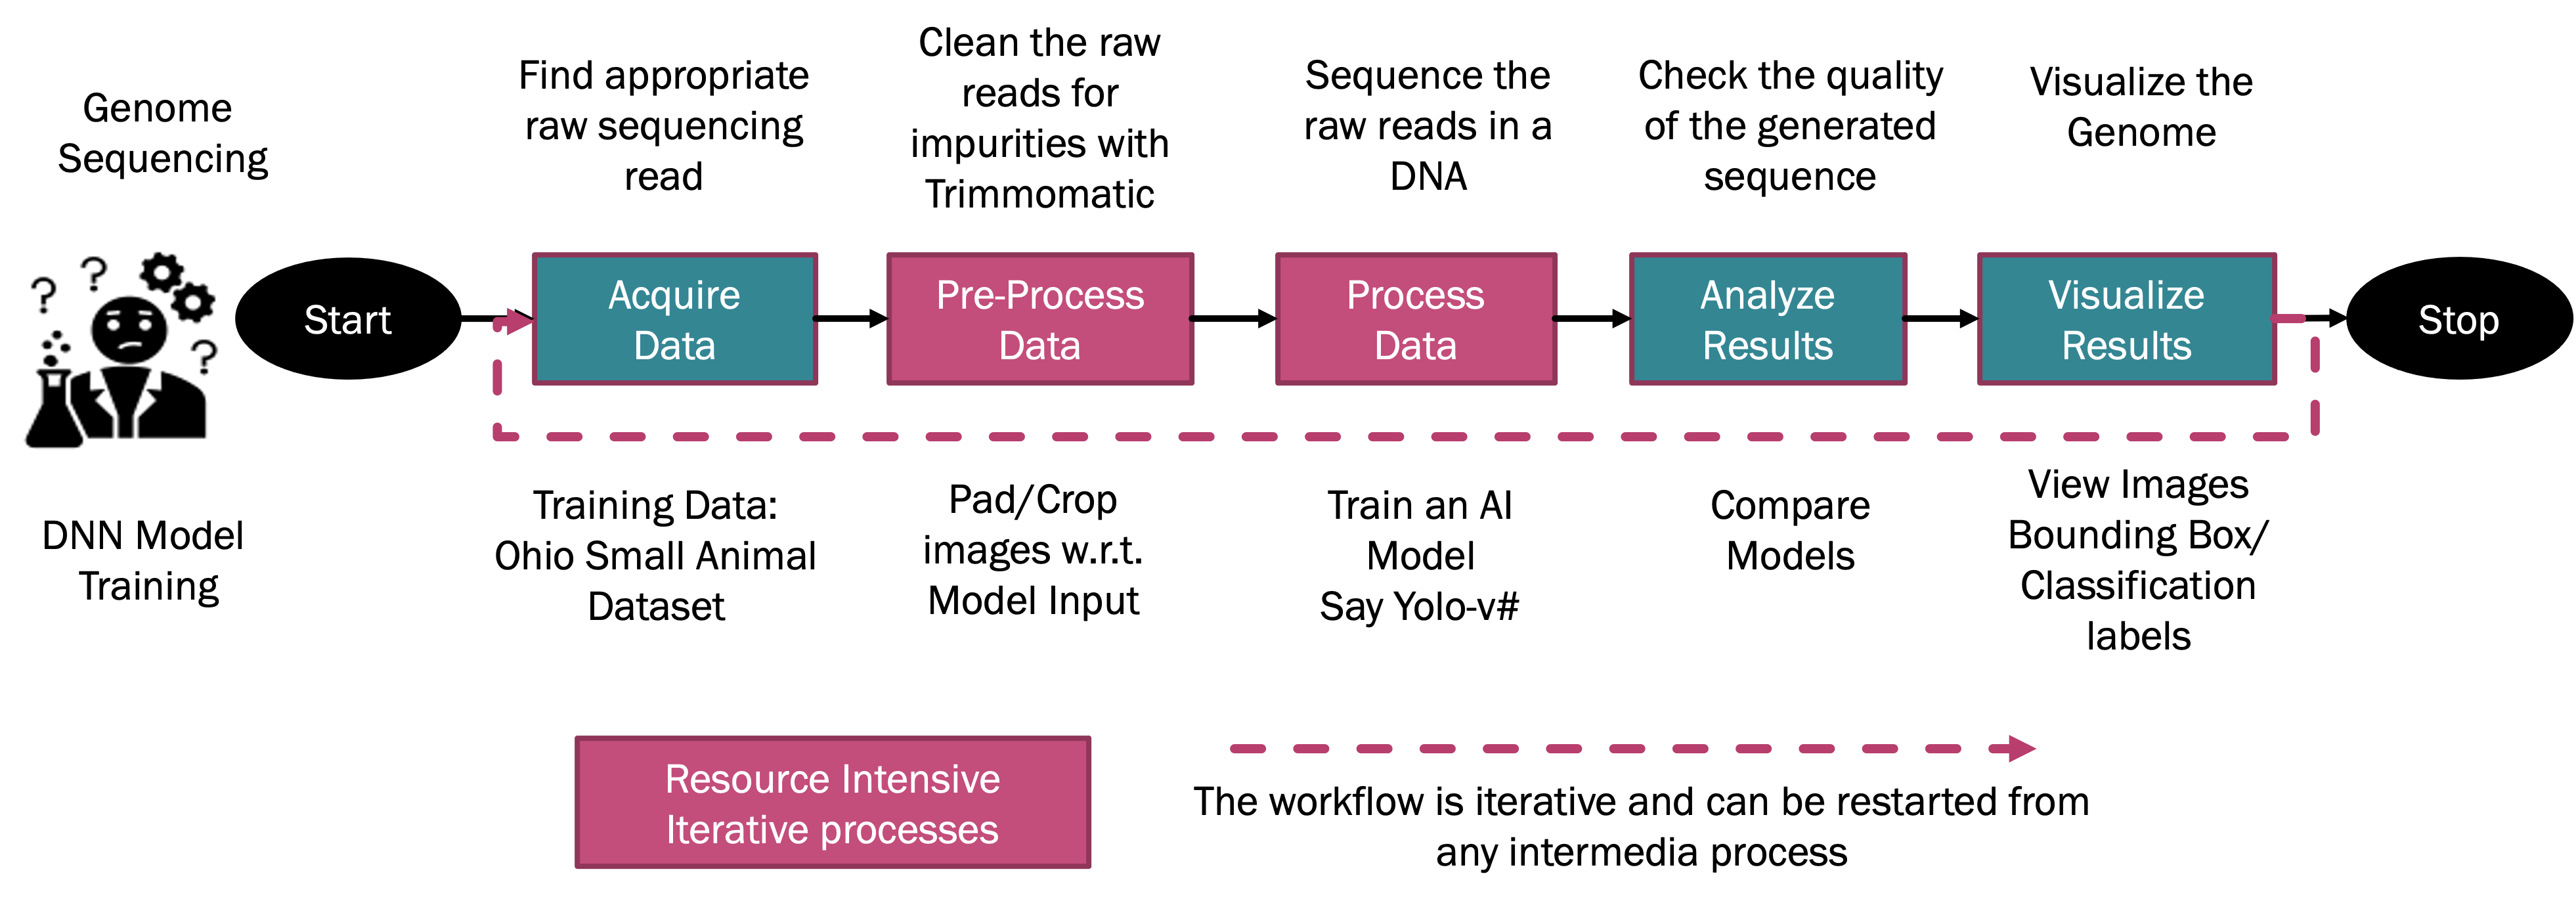
\includegraphics[width=0.8\textwidth]{Images/Workflow_overview.png}  % Adjust width as needed
    \caption{Overview of a Data-Driven Computational Workflow for Genome Assembly and DNN Training Pipelines}
    \label{fig:ExampleWorkFlows}
\end{figure}

These three applications were chosen to represent different points in the HPC application spectrum, considering variations in compute intensity, input-output (I/O) demands, and memory requirements.

\begin{itemize}
    \item Gray-Scott (Chemical Diffusion Simulator): This application simulates chemical diffusion based on Gray-Scott equations, using a 3D array to model the interaction of two reacting substances over a range of time steps. It takes parameters such as diffusion coefficients, reactant densities, feed/kill rates, and simulation steps. Since it performs intensive array manipulations to simulate diffusion dynamics, it is classified as compute-intensive.
    \item Trimmomatic (Genome Sequencing Preprocessing): Pre-cleaning is a critical step in genome sequencing and assembly to improve the quality of results. Trimmomatic is a widely used tool for removing impurities from Illumina short reads by trimming or filtering out low-quality bases while retaining high-quality ones. The application reads raw sequencing data, processes it, and writes the cleaned data back to storage. Due to its frequent read/write operations alongside computational processing, Trimmomatic is both compute- and I/O-intensive.
    \item Deep Neural Networks (DNNs) for Image Classification: We evaluated three large Convolutional Neural Network (CNN) models—VGG16, ResNet50, and InceptionV3—using the Keras API on TensorFlow. Each model contains millions of tunable parameters and requires loading the training data as RGB values into memory before initialization and training. Due to the high computational load and large memory footprint required for model execution, these applications are categorized as both compute- and memory-intensive.
\end{itemize}
This selection provided us a different spectrum of HPC workloads, covering compute-bound, I/O-bound, and memory-bound applications, enabling a diverse analysis of resource interactions in high-performance environments. Figure \ref{fig:ExampleWorkFlows} presents a general pipeline for data-driven computational workflows, while Figure \ref{fig:Mindmap} provides a mind map outlining various tools, datasets, and execution endpoints associated with different workflows 

\begin{figure}[h]
    \centering
    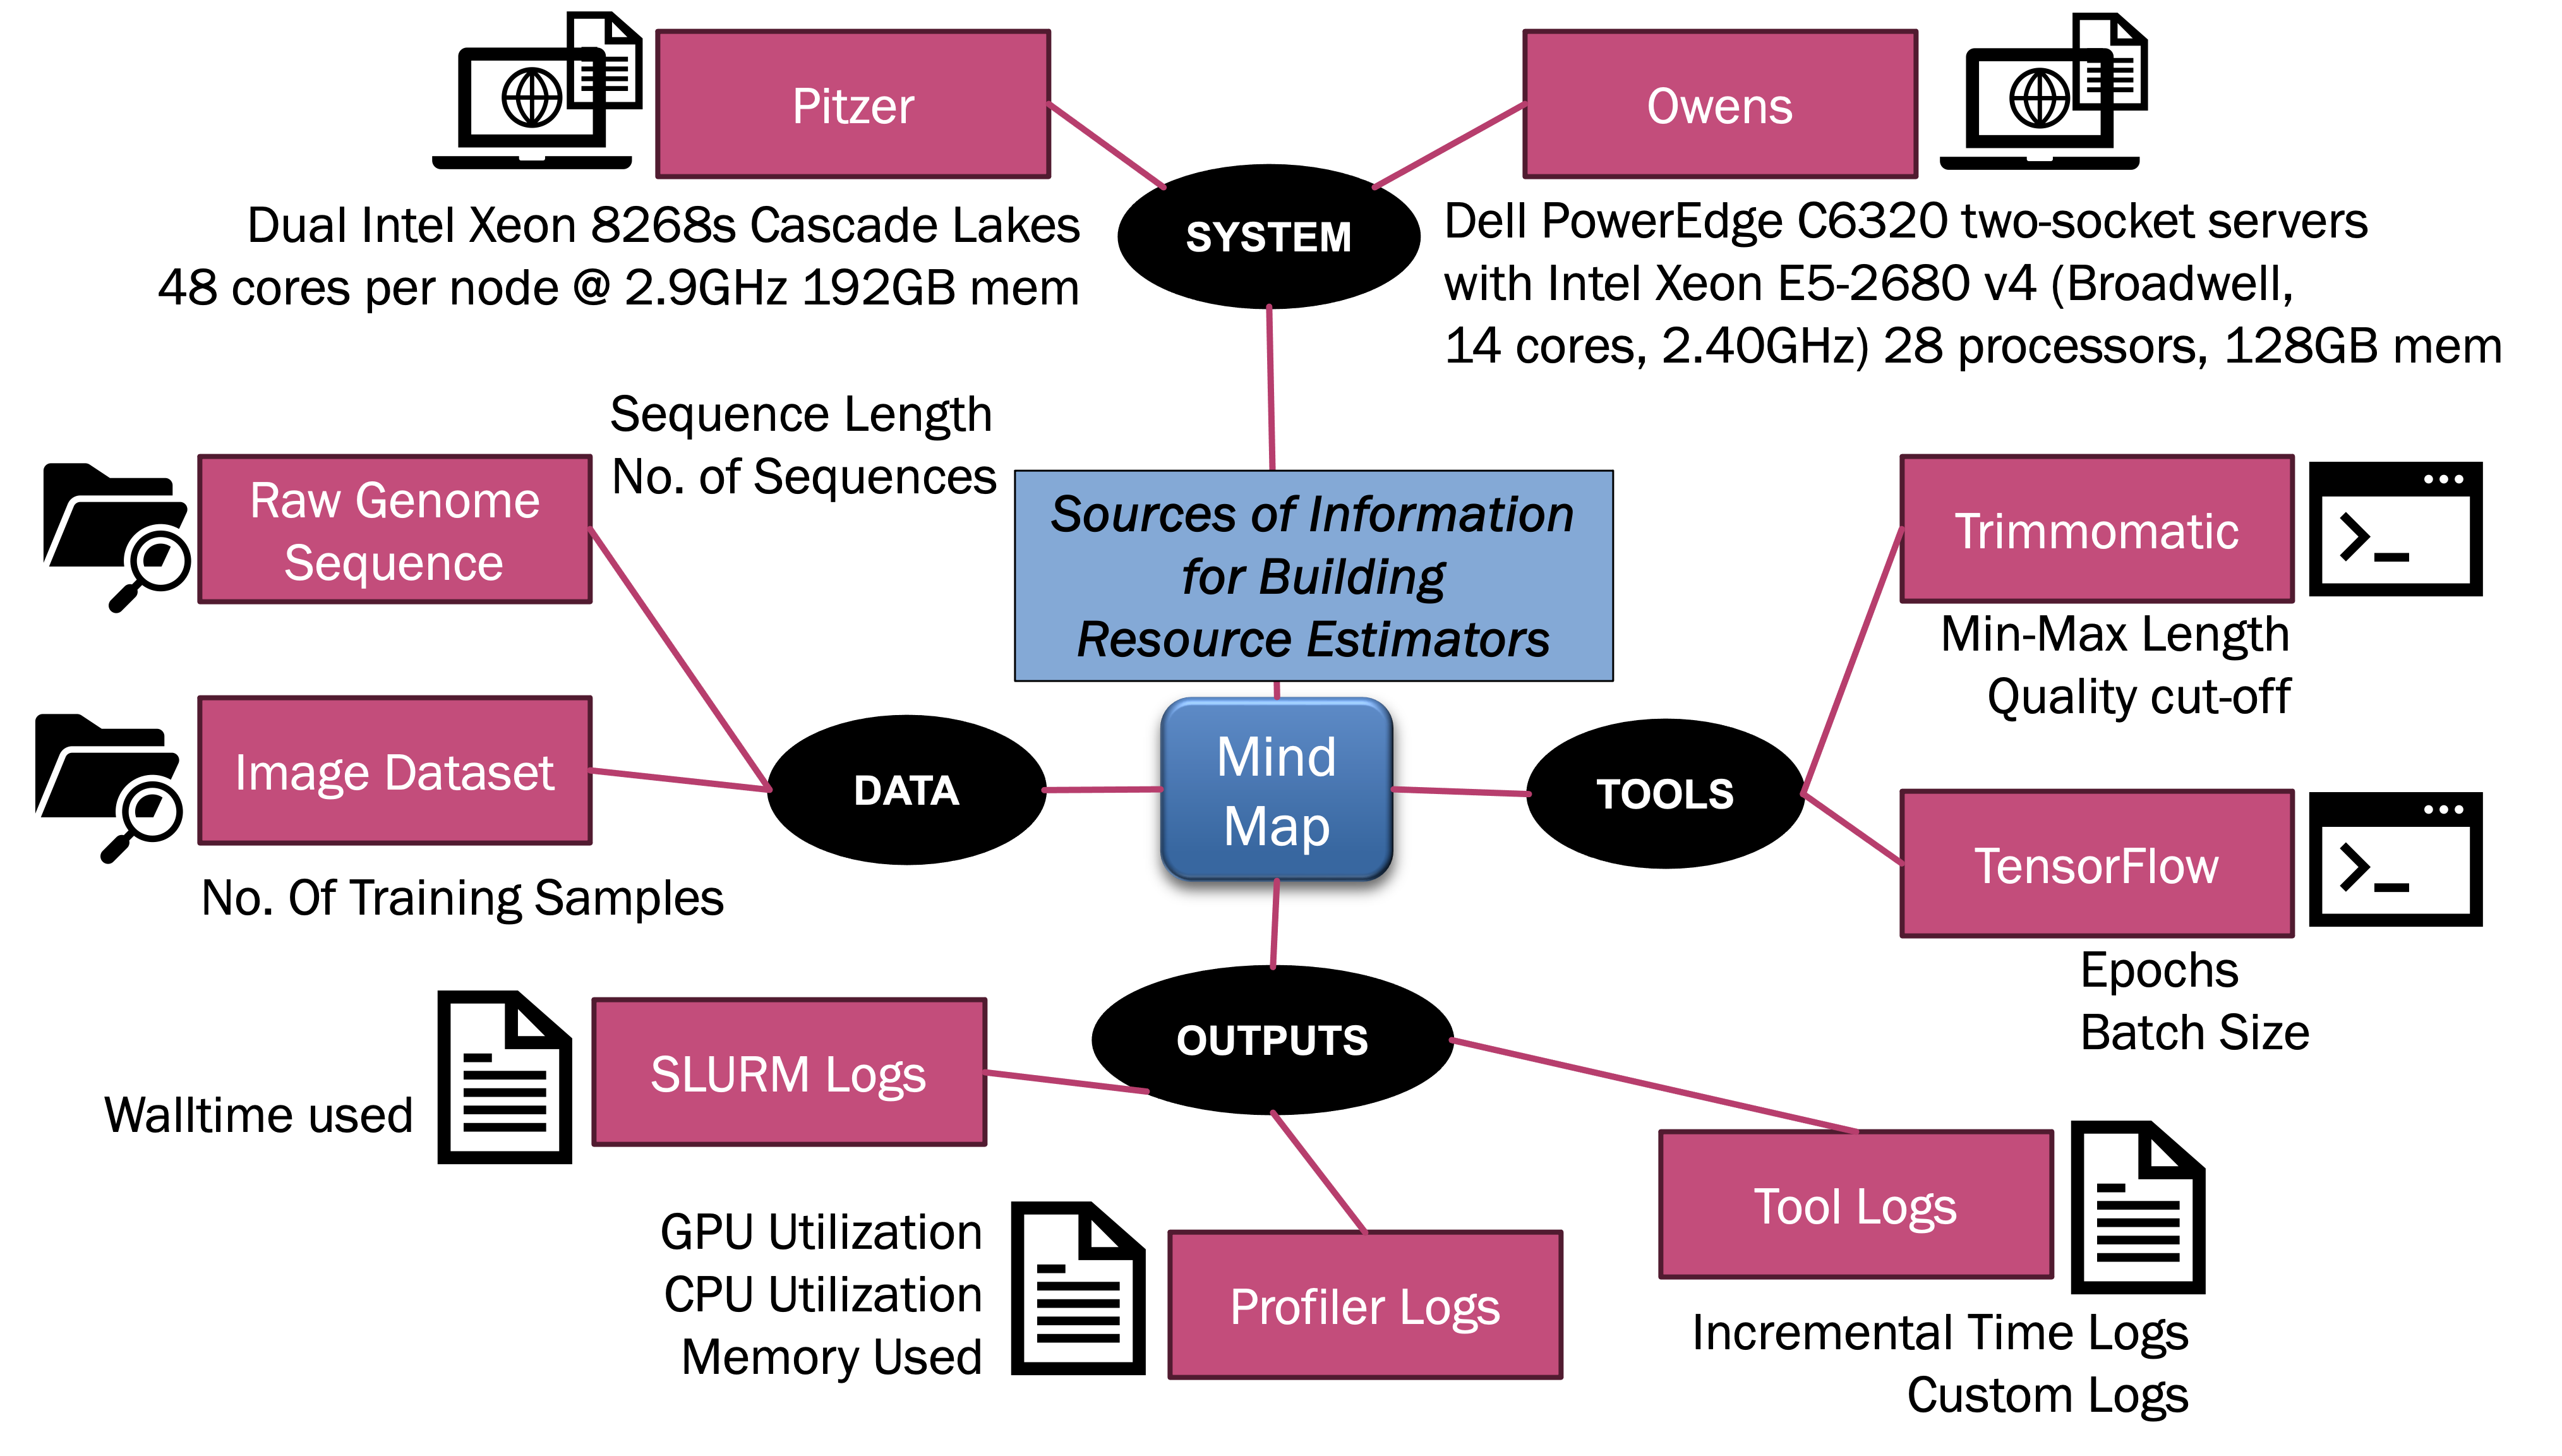
\includegraphics[width=0.8\textwidth]{Images/MindMap.png}  % Adjust width as needed
    \caption{Mind Map of Data, Tools, and System Components for Genome Assembly and DNN Training Workflows}
    \label{fig:Mindmap}
\end{figure}

\section{Challenges in HPC Resource Provisioning}

\begin{figure}[h]
    \centering
    \includegraphics[width=0.9\textwidth]{Images/JobAllocation.png}
    \caption{Workflow for Job Allocation, Execution, and Optimization in HPC Environments}
    \label{fig:job_allocation}
\end{figure}

Figure \ref{fig:job_allocation} illustrates the HPC job allocation and optimization workflow using SLURM and Grafana for job scheduling. The process begins with creating allocation scripts, which are either generated based on OSC Batch example documentation or adapted from peer-shared templates. Users typically analyze execution logs and Grafana metrics only when a job fails, diagnosing inefficiencies and adjusting resource allocations accordingly. However, resource fine-tuning is rarely performed for successfully executed jobs, even when it could reduce execution costs or improve scalability (as shown in Figure \ref{fig:log_tracking}). Job efficiency is assessed by monitoring CPU, memory, and GPU utilization using tools such as Grafana or XDMoD.

During these workloads, HPC users—regardless of their expertise with supercomputers—face several common challenges, including:

\begin{itemize}
    \item Job Termination Due to Resource Under-Provisioning: If a job exceeds the allocated walltime, it gets terminated, and without checkpointing, all progress is lost, leading to costly reruns. SLURM doesn't allow general users to extend their allocation during job execution. 
    \item Out-of-Memory (OOM) Errors for DNN Training on GPUs: Training a deep neural network (DNN), such as Inception V3, with a large batch size (e.g., 256) on a P100 GPU (which has 15.1 GB of usable memory out of 16 GB) can exceed memory limits, causing the job to fail.
    \item Difficulty in Fine-Tuning CPU Allocation for GPU-Centric Workloads: Users struggle to determine the optimal CPU allocation needed for data preprocessing during GPU training without impacting overall training time.
    \item Lack of Understanding in Interpreting Grafana Logs for CI Policies: Users face challenges in tuning --ntasks-per-node (no. of CPU cores) based on CPU memory requirements. For example, on Owens (where max memory per core is 4.214 GB), a workflow requiring 30 GB of memory should request at least 8 CPU cores to accommodate the workload efficiently.
    \item Policy Variations in Cyber-Infrastructure (CI) Allocations: \begin{itemize}
        \item At OSC, users can request partial nodes, enabling node sharing to accommodate multiple users simultaneously. When users submit job requirements (CPU cores, memory, GPUs, walltime) to SLURM, it dynamically assigns the job to an appropriate queue (e.g., serial, gpu-serial, hugemem, parallel, gpu-backfill).
        \item At TACC, node sharing is not enabled, meaning users must explicitly request a queue that best fits their workload. For example, the rtx-dev queue is used for short 2-hour jobs, while the rtx queue is allocated for 1-day jobs.
    \end{itemize}
    \item Need for Continuous Job Monitoring and Adaptive Scheduling: Users should actively monitor job execution to ensure it runs as expected. When necessary, jobs can be divided into smaller sub-jobs and scheduled either sequentially or strategically. This helps achieve faster allocation within the HPC batch queue system based on availability and ensures the jobs fit within queue limitations, improving overall computational efficiency.
\end{itemize}

\begin{figure}[h]
    \centering    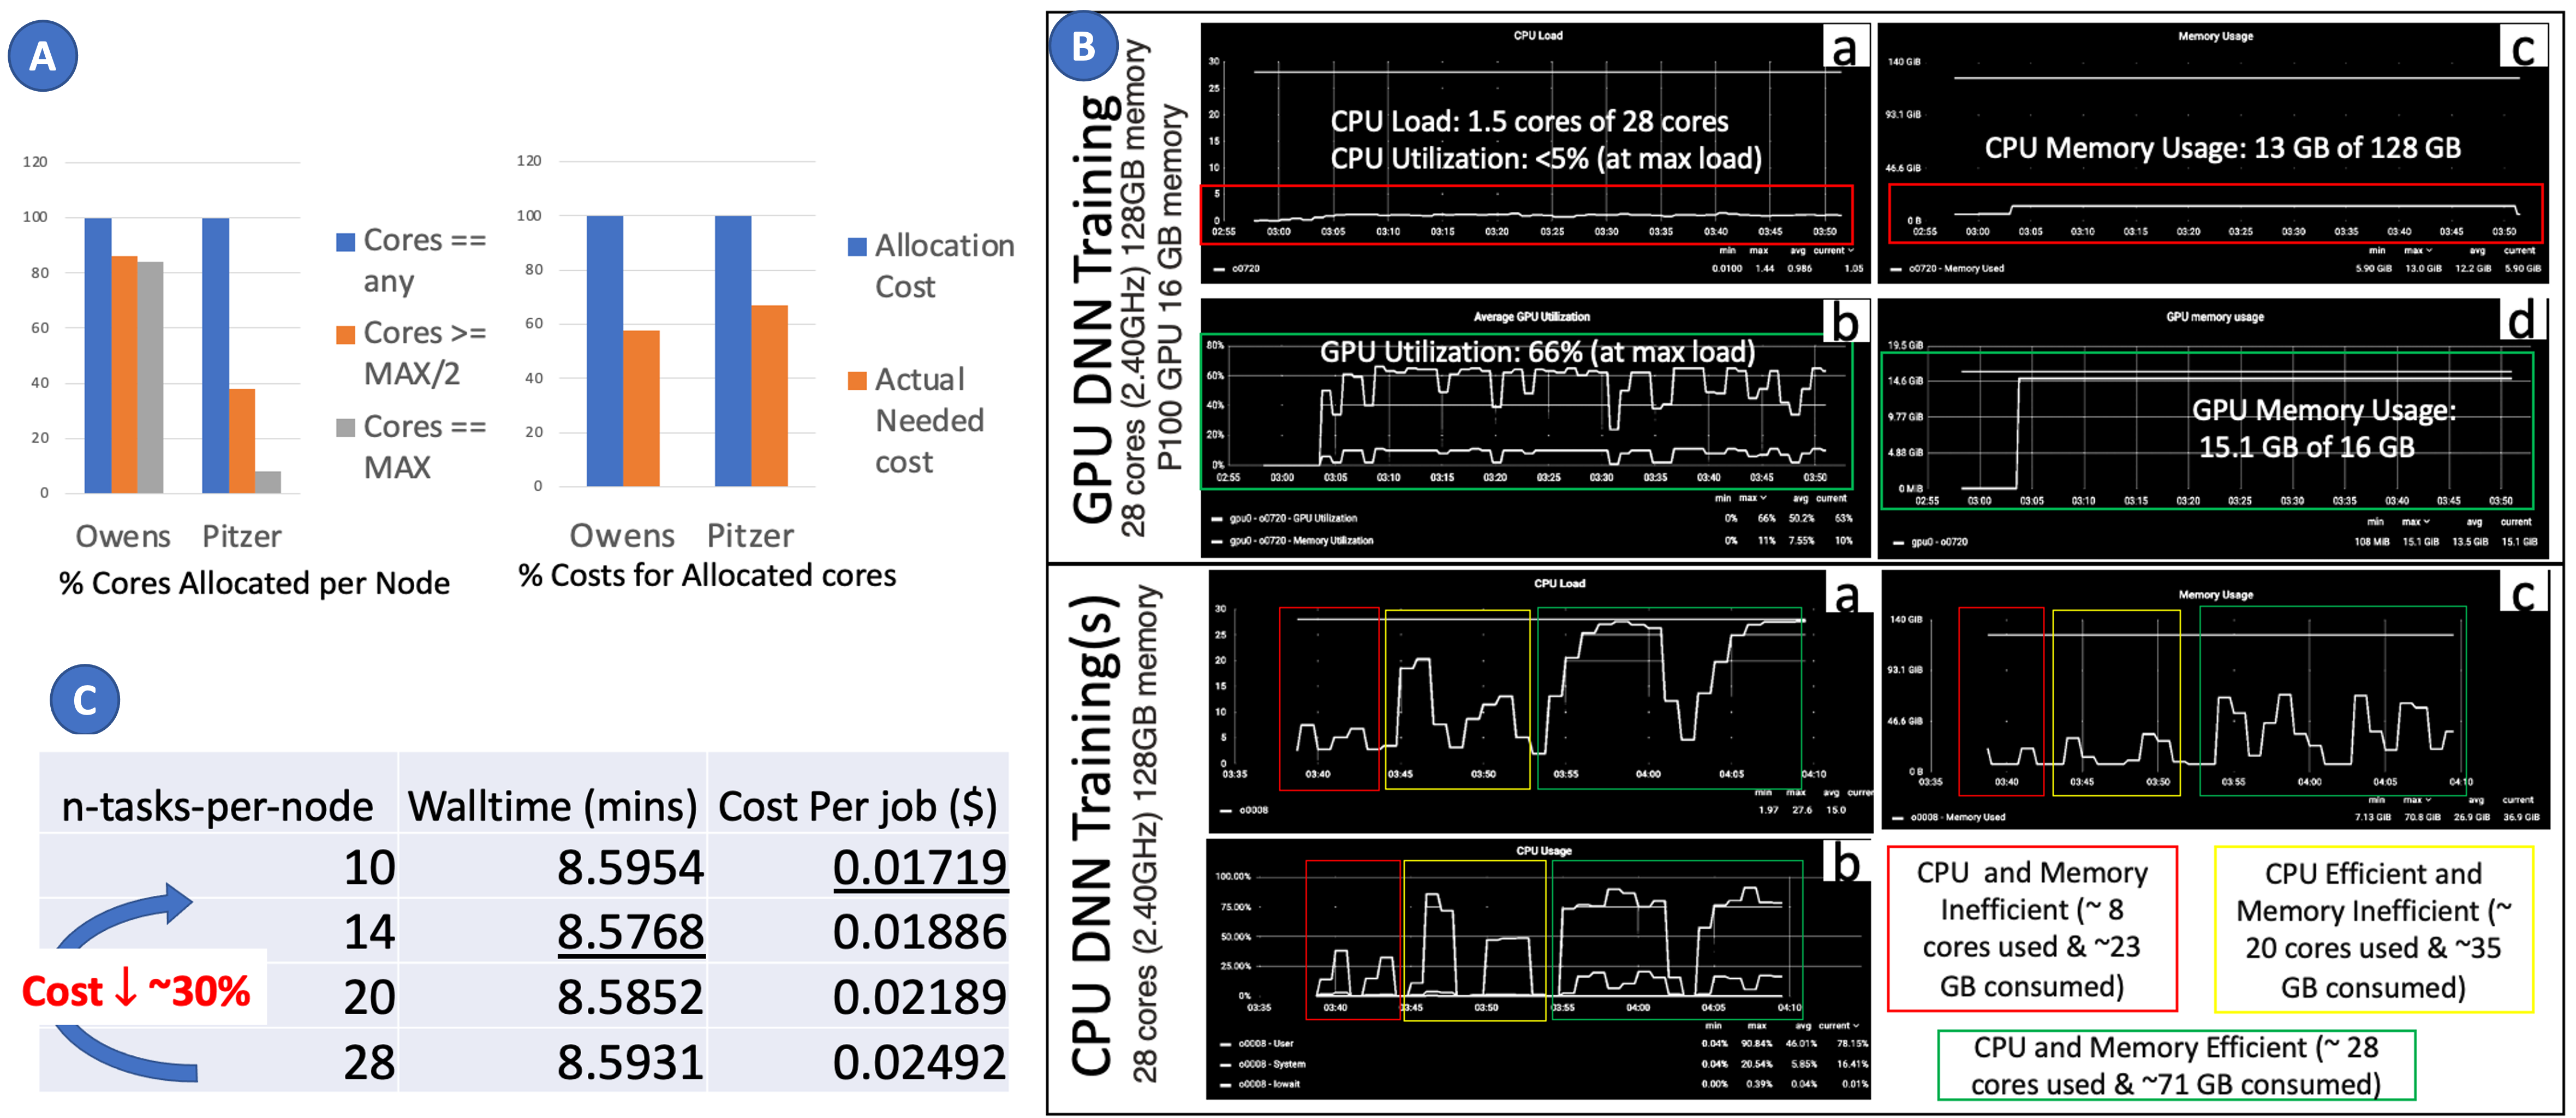
\includegraphics[width=1.0\textwidth]{Images/LogTracking.png}
    \caption{A snapshot of CPU and GPU Resource Utilization, Allocation Inefficiencies, and Cost Optimization in HPC Workloads. 
    % (A) Core Allocation and Cost Analysis: Comparison of allocated vs. needed cores on Owens and Pitzer, highlighting differences in resource usage and cost. (B) GPU DNN Training Metrics: Grafana logs showing CPU load, GPU utilization, and memory usage, demonstrating inefficiencies in CPU allocation for DNN training on a P100 GPU and variations based on hyperparameters. (C) Cost Optimization: Adjusting n-tasks-per-node reduces unnecessary CPU allocation, lowering costs by ~30\% without affecting wall time.
    }
    \label{fig:log_tracking}
\end{figure}

Figure \ref{fig:log_tracking} provides an overview of CPU and GPU resource utilization, allocation inefficiencies, and cost optimization for HPC workloads. (A) Core Allocation and Cost Analysis compares allocated versus required CPU cores on Owens and Pitzer supercomputers, highlighting disparities in resource allocation and the associated costs. The analysis demonstrates how over-provisioning leads to unnecessary expenses. (B) GPU DNN Training Metrics presents Grafana logs showcasing CPU load, GPU utilization, and memory consumption during deep neural network (DNN) training on a P100 GPU. It highlights inefficiencies in CPU allocation and illustrates how resource demands fluctuate based on DNN hyperparameters. (C) Cost Savings with Optimal CPU Allocation examines the impact of adjusting n-tasks-per-node to improve CPU efficiency. The results indicate that reducing excess core allocation can lower costs by ~30\% without increasing wall time, demonstrating the importance of resource-aware job scheduling in HPC environments.


\section{Key Research Questions}
\label{Sec:Problem_KeyReserachQuestions}

By analyzing \textbf{user-HPC interaction endpoints and workload patterns}, as outlined above, this thesis aims to develop \textbf{software and ML-based solutions} to enhance \textbf{resource allocation and utilization}. The proposed approaches address the following key research questions:  

\textbf{Question 1: Can AI models be used to develop resource estimators for predicting runtime and memory feasibility for user-specific jobs?}  

\begin{itemize}
    \item \textbf{What datasets are available or needed} to train models that estimate job-specific resources? If none exist, how can they be efficiently created?  
    \item \textbf{What features should be captured} to predict resource requirements, such as runtime or memory?  
    \item \textbf{Which models} can best predict resource requirements? Can a \textbf{"one model fits all"} approach work across different workflows and estimations (e.g., memory, walltime)?  
    \item \textbf{Can standard ML metrics} like \textbf{mean squared error (MSE)} be used to validate resource estimations, or do we need \textbf{custom evaluation metrics}?  
\end{itemize}


\textbf{Question 2: Can a framework be designed to integrate these estimators into a SLURM wrapper, enabling automated job submission, tracking, and execution based on resource availability and CI batch policy limitations?}

\begin{itemize}
    \item \textbf{Can we create a multi-purpose cyberinfrastructure database} that helps:  
    \begin{itemize}
        \item Users understand all \textbf{available queues} and their limitations?  
        \item Estimate the \textbf{cost of allocations} based on job configurations?  
        \item Assess \textbf{execution feasibility} and dynamically configure scheduling?  
    \end{itemize}
    \item \textbf{Can long-running jobs be tracked} using \textbf{SLURM or tool logs}? What ecosystem is required to monitor job progress and efficiency?  
\end{itemize}

In Chapter \ref{Background.ch}, we examine existing solutions that address the aforementioned questions and identify the bottlenecks that serve as the driving factors for our research.




